\documentclass[12pt, a4paper,twoside]{tesi_upf}


%CODIFICACI�
\usepackage[latin1]{inputenc}


%IDIOMES
\usepackage[catalan,english]{babel}

%NOM�S PER A OBTENIR INDICACI� DEL MARC EN MIDA A4
\usepackage[cam,a4,center,frame]{crop}

%PER A INCLOURE GR�FICS I EL LOGO DE LA UPF
\usepackage{graphicx}
\usepackage{caption}

%FONTS TIMES O GARAMOND, 
\usepackage{times}
%\usepackage{garamond}

%SENSE HEADINGS: NO MODIFICAR
\pagestyle{plain}

%PER A L'�NDEX DE MAT�RIES
\usepackage{makeidx}
\makeindex

%ESTIL DE BIBLIOGRAFIA
\bibliographystyle{apalike}


%AQUEST DOCUMENT �S EN CATAL�
\selectlanguage{english}

%EN COMPTES DE �NDEX, LA TAULA DE CONTINGUTS ES TITULA SUMARI
\addto\captionscatalan
  {\renewcommand{\contentsname}{\Large \sffamily Sumari}}


%AFEGIU EN AQUESTA PART LES VOSTRES DADES
\title{El t�tol de la tesi: Obligatori}
\subtitle{El subt�tol de la tesi: Opcional}
\author{Autor: Obligatori}
\thyear{L'any de la tesi: Obligatori}
\department{Departament: Obligatori}
\supervisor{Director: Obligatori}


\begin{document}


\frontmatter

\maketitle

\cleardoublepage


%%%%%% Dedicat�ria; si no es vol posar, comenteu fins a final de dedicat�ria

\noindent Escriviu aqu� la vostra dedicat�ria

\cleardoublepage

%%%%%% Final de dedicat�ria


%%%%%% Agra�ments; si no es vol posar, comenteu fins a final de agra�ments
\noindent {\Large \sffamily Agra�ments} Agraeixo....

\cleardoublepage

%%%%%% Final dels agra�ments

%ABSTRACT EN DOS IDIOMES. COM A M�NIM CATAL�. SI L'ALTRE �S EN CASTELLA CANVIEU EL QUE POSA ABSTRACT
\selectlanguage{english}
\section*{\Large \sffamily Abstract}
This is the abstract of the thesis in English.  Please, use less
than 150 words.

\selectlanguage{catalan}
\vspace*{\fill}
\section*{\Large \sffamily  Resum}
Vet aqu� el resum de la tesi en catal�.  Si us plau, utilitzeu
menys de 150 paraules.
\vspace*{\fill}

\selectlanguage{english}
\cleardoublepage
%FIN DE ABSTRACTE

%PREFACI OPCIONAL. SI NO ES VOL, COMENTEU FINS EL FINAL DE PREFACI
{\bf Prefaci}

\cleardoublepage
%FINAL DE PREFACI


%TAULA DE CONTINGUTS: OBLIGAT�RIA
\tableofcontents

%INDEX DE FIGURES; NOM�S ES POSA SI HI HA FIGURES
\listoffigures
%Fa que aparegui al sumari
\addcontentsline{toc}{chapter}{List of figures}

%INDEX DE TAULES; NOM�S ES POSA SI HI HA TAULES
\listoftables
%Fa que aparegui al sumari
\addcontentsline{toc}{chapter}{List of tables}

%COMEN�A EL TEXT
\mainmatter
\chapter{Introduction}
TODO
\chapter{State of the Art}

This project consists on studying how are, currently, being build  the open mesh networks in cities and what mechanisms we have to contribute or improve them. There are many different ways to improve this networks, namely, we can use different hardware, different software, build applications which run over them, etc.

First of all, we will analyze how these networks are, and how are they operating to have a better idea of what we want to improve.

\section{Mesh and MANET networks}

\subsection{Definition and properties}

When we talk about mesh networks, we refer to networks where all the participant are also routers. If we had to set a single definition the following can be a good one:
\\[10pt]
"\textit{A Mesh network is one where all nodes (participants) are routers, meaning that all the nodes accept and forward packets from other nodes according to the routing rules.}" \cite{paupfc}
\\[12pt] 
%Acronimo para a�adir
More specifically, we want to talk about Wireless Mesh Networks (WMN) which may refer also to the users of the network, and can be defined as follows:
\\[10pt]
"\textit{Wireless mesh networks often consist of mesh clients, mesh routers and gateways. The mesh clients are often laptops, cell phones and other wireless devices while the mesh routers forward traffic to and from the gateways which may but need not connect to the Internet.}" \cite{huynhsimulation}
\\[12pt]

To summarize, we have that mesh networks are basically networks which are not defined by the topology (physical layer) or the kind of links between two nodes (link layer). They are defined by the way the nodes operate among them, there are not master/slave or node/supernode distinctions and so, all the nodes have a similar function. In addition, the clients (end users) do not notice any difference (between mesh or other kind of networks) when they connect to the mesh, they are totally transparent for them. 
\\[12pt]

As mentioned above, there are only two different kind of nodes: mesh routers and mesh gateways. They operate in exactly the same way when they have to route packets within the network, the only difference is that the gateways may be connected to a wider network, namely, the Internet and they can route packets to this other network. So, mesh routers just route packets inside the mesh while mesh gateways can also route packets to the outside. 
\\[12pt]

	\noindent%
\begin{minipage}{\linewidth}
\vspace{10 mm}
\makebox[\linewidth]{%
  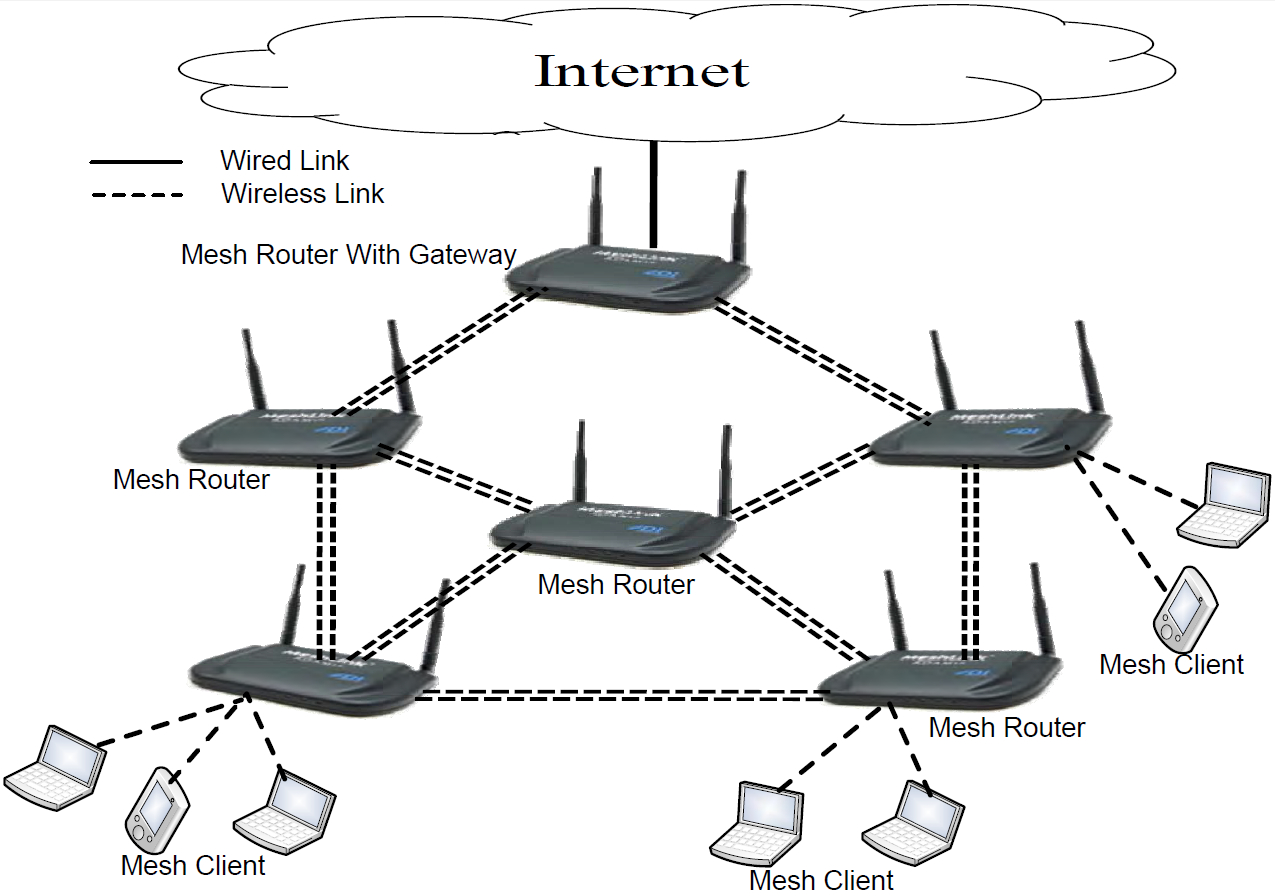
\includegraphics[width=0.8 \linewidth]{Images/wmn11.jpg}}
\captionof{figure}{Wireless Mesh Network Example}% only if needed
\caption*{http://www.intechopen.com/source/html/37888/media/wmn11.jpg}
\label{city}
\end{minipage}
\nocite{WMNs}
\clearpage

Then, we can say that WMN are a subtype of mesh networks. They have all the properties of these networks with the only difference that all the nodes are connected wirelessly. 

\subsection{Operating modes}



     



\chapter{Methodology}
TODO
\chapter{Contribution}

\chapter{Results}
TODO
\chapter{Conclusions}
TODO
\chapter{Future Work}
TODO






\bibliography{bibliography}



\backmatter
\printindex





\end{document}


%NUMERACI� DE LA P�GINA EXTERIOR EXCEPTE EN LA PRIMERA P�GINA DE CADA CAP�TOL
\usepackage{fancyhdr}
\pagestyle{fancy}
\fancyfoot{}
\fancyfoot[RO]{\thepage}
\fancyfoot[LE]{\thepage}


%MUTIPLES �NDEX
%En el pre�mbul
\usepackage{multind}
\makeindex{authors}
%Introducci� d'entrades la forma
\index{authors}{Einstein}
%Situaci� de l'�ndex
\printindex{authors}{Author index}
%Cal eliminar les comandes \usepakage{makeidx} \makeindex \printindex
%cal exacutar des de la l�nia de comandes makeindex authors